\chapter{Experimental Results}
\label{chapter:results}

This chapter summarises the results of our experiment assessing sixteen resampling methods over
eighteen datasets. Sixteen of these datasets are publicly available on OpenML~\cite{openml}. The
remaining two datasets, namely \emph{Graph - Embedding} and \emph{Graph - Raw}, are proprietary
cyber security datasets. We can see the datasets' names, sizes and imbalances in
Table~\ref{table:datasets}.

\begin{table}
    \centering

    \begin{tabular}{lrrrr}
        \toprule
        Name & Size & Majority Size & Minority Size & Imbalance \\
        \midrule
        Asteroid & 126131 & 125975 & 156 & 807.532 \\
        Credit Card Subset & 14240 & 14217 & 23 & 618.130 \\
        Credit Card & 284807 & 284315 & 492 & 577.876 \\
        PC2 & 5589 & 5566 & 23 & 242.000 \\
        MC1 & 9466 & 9398 & 68 & 138.206 \\
        Employee Turnover & 34452 & 33958 & 494 & 68.741 \\
        Satellite & 5100 & 5025 & 75 & 67.000 \\
        BNG - Solar Flare & 663552 & 648320 & 15232 & 42.563 \\
        Mammography & 11183 & 10923 & 260 & 42.012 \\
        Letter & 20000 & 19187 & 813 & 23.600 \\
        Relevant Images & 134731 & 129149 & 5582 & 23.137 \\
        Click Prediction V1 & 1496391 & 1429610 & 66781 & 21.407 \\
        Click Prediction V2 & 149639 & 142949 & 6690 & 21.368 \\
        Amazon Employee & 32769 & 30872 & 1897 & 16.274 \\
        BNG - Sick & 1000000 & 938761 & 61239 & 15.329 \\
        Sylva Prior & 14395 & 13509 & 886 & 15.247 \\
        BNG - Spect & 1000000 & 915437 & 84563 & 10.826 \\
        \bottomrule
    \end{tabular}

    \caption{
        \textbf{Public Datasets.} The table shows basic information about public datasets used in
        the experiments.
    }
    \label{table:datasets}
\end{table}


Besides sixteen resampling methods, we also include a no-op preprocessing method to obtain baseline
results on the original datasets without performing any preprocessing. The resampling methods and
the number of possible configurations of the hyperparameters we search through are summarised in
Table~\ref{table:configs}.

\begin{table}
    \centering

    \begin{tabular}{lr}
        \toprule
        Method & Hyperparameter Configurations \\
        \midrule
        Baseline & 1 \\
        Random Oversampling & 2 \\
        SMOTE & 4 \\
        Borderline SMOTE & 16 \\
        SVM SMOTE & 8 \\
        KMeans SMOTE & 4 \\
        ADASYN & 4 \\
        Random Undersampling & 2 \\
        CNN & 2 \\
        ENN & 4 \\
        Repeated ENN & 4 \\
        All KNN & 4 \\
        Near Miss & 12 \\
        Tomek Links & 1 \\
        One-Sided Selection & 2 \\
        NCL & 8 \\
        Cluster Centroids & 4 \\
        \midrule
        $\Sigma$ & 82 \\
        \bottomrule
    \end{tabular}

    \caption{
        \textbf{Hyperparameter Configurations for Preprocessing Methods.} The table shows the
        number of available hyperparameter configurations in the experiments.
    }
    \label{table:configs}
\end{table}


We report the results using eight evaluation metrics. Concretely, Balanced Accuracy, Precision,
Recall and Matthews Correlation Coefficient with the default decision threshold set to 0.5; F1 Max
with a decision threshold maximising the score on the testing set; Area Under the Precision-Recall
(PR) and Receiver Operating Characteristics (ROC) curves and lastly area under the partial ROC
curve with FPR values on the horizontal axis ranging from 0 to the imbalance ratio of the
corresponding dataset.

Eighteen separate tables are included for each dataset providing detailed metrics for each
preprocessing method in Appendix~\ref{appendix:scores}. Maximal values of each metric are
highlighted in bold font. Some of the tables contain unsuccessful runs labelled \emph{N/A}. The
most common reason for failure was a substantial amount of time needed to resample the dataset and
insufficient time to train a classifier on large datasets.

We include a table containing average ranks for each combination of preprocessing method and
evaluation metric computed across all datasets~\ref{table:mean-rank}. Ranks are computed as
follows: the highest score is assigned a rank of 1, the second-highest a rank of 2 and so on.
Average ranks are assigned in case of ties. Some of the preprocessing methods did not finish
successfully on specific datasets; thus, the second number in each cell represents the number of
datasets across which the average rank was computed. However, many of the preprocessing methods
still finished successfully on all datasets with one exception. We can see that the KMeans SMOTE
preprocessing method successfully finished only on four datasets due to exceptions interrupting the
resampling process.

The table also shows that oversampling methods were ranked better on average than undersampling
methods when considering the P-ROC metric. We include a violin plot in
Figure~\ref{figure:p-roc-ranks} showing the distribution of ranks for each resampling method when
evaluated using the P-ROC score to explore this hypothesis more. We also include the same plot for
all other evaluation metrics in Appendix~\ref{appendix:distributions}. It is even more clear from
the figure that, indeed, the oversampling methods (methods from Random Oversampling to ADASYN)
achieved better ranks than undersampling methods. However, there are some exceptions within the
group of undersampling methods. Random Undersampling and Cluster Centroids consistently achieved
ranks comparable to those of oversampling methods. Condensed Nearest Neighbour, Edited Nearest
Neighbours and NearMiss did not reach the scores of oversampling methods but outperformed the
baseline method, i.e. no preprocessing at all. The remaining undersampling methods achieved
approximately the same performance as the baseline.

We also performed the Friedman test which is a non-parametric equivalent of repeated-measures
ANOVA~\cite{stats-comparison}. The Friedman test assigns ranks to each method in the same way we
discussed above and it compares average ranks of the methods. The null hypothesis states that all
algorithms participating in the test are equivalent and thus have the same average rank. We
rejected the null hypothesis at 0.001 significance level under all eight evaluation metrics,
supporting our previous claim that some preprocessing methods achieved better ranks than others.

Furthermore, we include a violin plot showing the distribution of preprocessing times of each
resampling method together with the mean value, 25th, 50th and 75th percentile in
Figure~\ref{figure:preprocessing-times}. Even in this case, oversampling methods achieved slightly
better times than undersampling methods. Understandably, Random Oversampling and Undersampling took
the least amount of time as they do not perform any heavy computations. KMeans SMOTE seems to be
faster than any of the remaining preprocessing methods. However, we need to keep in mind that
KMeans SMOTE finished successfully only on four datasets, out of which two contained only a couple
hundred samples. Forgetting about these preprocessing methods gives way to the SMOTE. It is evident
from the results why SMOTE is considered the most widely used resampling method. It achieved one of
the best ranks and performed resampling much faster than other preprocessing methods.

We see that an excellent distribution of ranks of Cluster Centroids may be negated by the amount of
time it needs to resample the datasets putting it in line with other undersampling methods. Lastly,
two resampling methods stand out from the crowd negatively. SVM SMOTE and Condensed Nearest
Neighbour methods were the slowest methods in our experiments, peaking with a maximum resampling
time of over a day.

\clearpage
\begin{table}
    \centering
    \setlength\tabcolsep{2pt}
    \renewcommand\arraystretch{0.95}
    \widesplit{
        \makebox[\textwidth]{
            \begin{tabularx}{\textwidth}{lRRRR}
                \toprule
                & \row{B. Accuracy & Precision & Recall & F1 Max}{PR AUC & MCC & ROC AUC & P-ROC AUC} \\
                \midrule
                Baseline & \row{12.472 // 18 & 7.528 // 18 & 12.667 // 18 & 7.750 // 18}{7.667 // 18 & 10.222 // 18 & 7.611 // 18 & 12.056 // 18} \\
                Random Oversampling & \row{8.278 // 18 & 8.417 // 18 & 9.361 // 18 & 7.333 // 18}{8.917 // 18 & 6.694 // 18 & 8.500 // 18 & 5.889 // 18} \\
                SMOTE & \row{6.139 // 18 & 7.500 // 18 & 7.917 // 18 & 6.083 // 18}{6.000 // 18 & 5.250 // 18 & 5.944 // 18 & 3.556 // 18} \\
                Borderline SMOTE & \row{7.250 // 14 & 4.929 // 14 & 9.071 // 14 & 5.250 // 14}{5.786 // 14 & 5.250 // 14 & 6.643 // 14 & 5.071 // 14} \\
                SVM SMOTE & \row{5.176 // 17 & 5.971 // 17 & 7.324 // 17 & 5.176 // 17}{4.765 // 17 & 3.912 // 17 & 5.000 // 17 & 3.294 // 17} \\
                KMeans SMOTE & \row{9.625 // 04 & 5.875 // 04 & 11.875 // 04 & 5.625 // 04}{4.500 // 04 & 4.375 // 04 & 2.875 // 04 & 4.000 // 04} \\
                ADASYN & \row{6.639 // 18 & 7.889 // 18 & 7.389 // 18 & 7.417 // 18}{7.972 // 18 & 6.583 // 18 & 7.667 // 18 & 4.833 // 18} \\
                Random Undersampling & \row{3.556 // 18 & 11.528 // 18 & 3.833 // 18 & 8.667 // 18}{9.111 // 18 & 8.444 // 18 & 8.417 // 18 & 4.972 // 18} \\
                CNN & \row{8.083 // 12 & 10.833 // 12 & 5.792 // 12 & 10.667 // 12}{12.000 // 12 & 9.500 // 12 & 11.833 // 12 & 9.083 // 12} \\
                ENN & \row{7.167 // 18 & 5.306 // 18 & 7.528 // 18 & 6.278 // 18}{6.444 // 18 & 5.944 // 18 & 5.972 // 18 & 9.250 // 18} \\
                Repeated ENN & \row{7.833 // 12 & 5.500 // 12 & 7.625 // 12 & 8.833 // 12}{7.958 // 12 & 7.542 // 12 & 7.667 // 12 & 11.875 // 12} \\
                All KNN & \row{9.462 // 13 & 7.192 // 13 & 8.500 // 13 & 8.154 // 13}{8.115 // 13 & 8.000 // 13 & 8.269 // 13 & 12.462 // 13} \\
                Near Miss & \row{7.278 // 18 & 12.278 // 18 & 2.250 // 18 & 11.083 // 18}{11.333 // 18 & 12.306 // 18 & 11.889 // 18 & 7.833 // 18} \\
                Tomek Links & \row{11.833 // 18 & 6.639 // 18 & 11.778 // 18 & 8.944 // 18}{7.417 // 18 & 9.972 // 18 & 7.417 // 18 & 11.861 // 18} \\
                One-Sided Selection & \row{12.417 // 18 & 6.944 // 18 & 12.472 // 18 & 8.583 // 18}{7.972 // 18 & 10.083 // 18 & 8.694 // 18 & 12.139 // 18} \\
                NCL & \row{9.143 // 14 & 8.643 // 14 & 8.607 // 14 & 8.357 // 14}{8.857 // 14 & 8.571 // 14 & 9.500 // 14 & 11.643 // 14} \\
                Cluster Centroids & \row{4.200 // 15 & 10.667 // 15 & 3.500 // 15 & 10.500 // 15}{9.133 // 15 & 10.133 // 15 & 9.000 // 15 & 4.967 // 15} \\
                \bottomrule
            \end{tabularx}
        }
    }
    \caption{
        \textbf{Mean Rank Across All Datasets.} The table contains average ranks for each
        combination of preprocessing method and evaluation metric computed across all datasets. The
        second number after \emph{//} indicates the number of datasets used to compute the average.
    }
    \label{table:mean-rank}
\end{table}


\begin{figure}
    \centering
    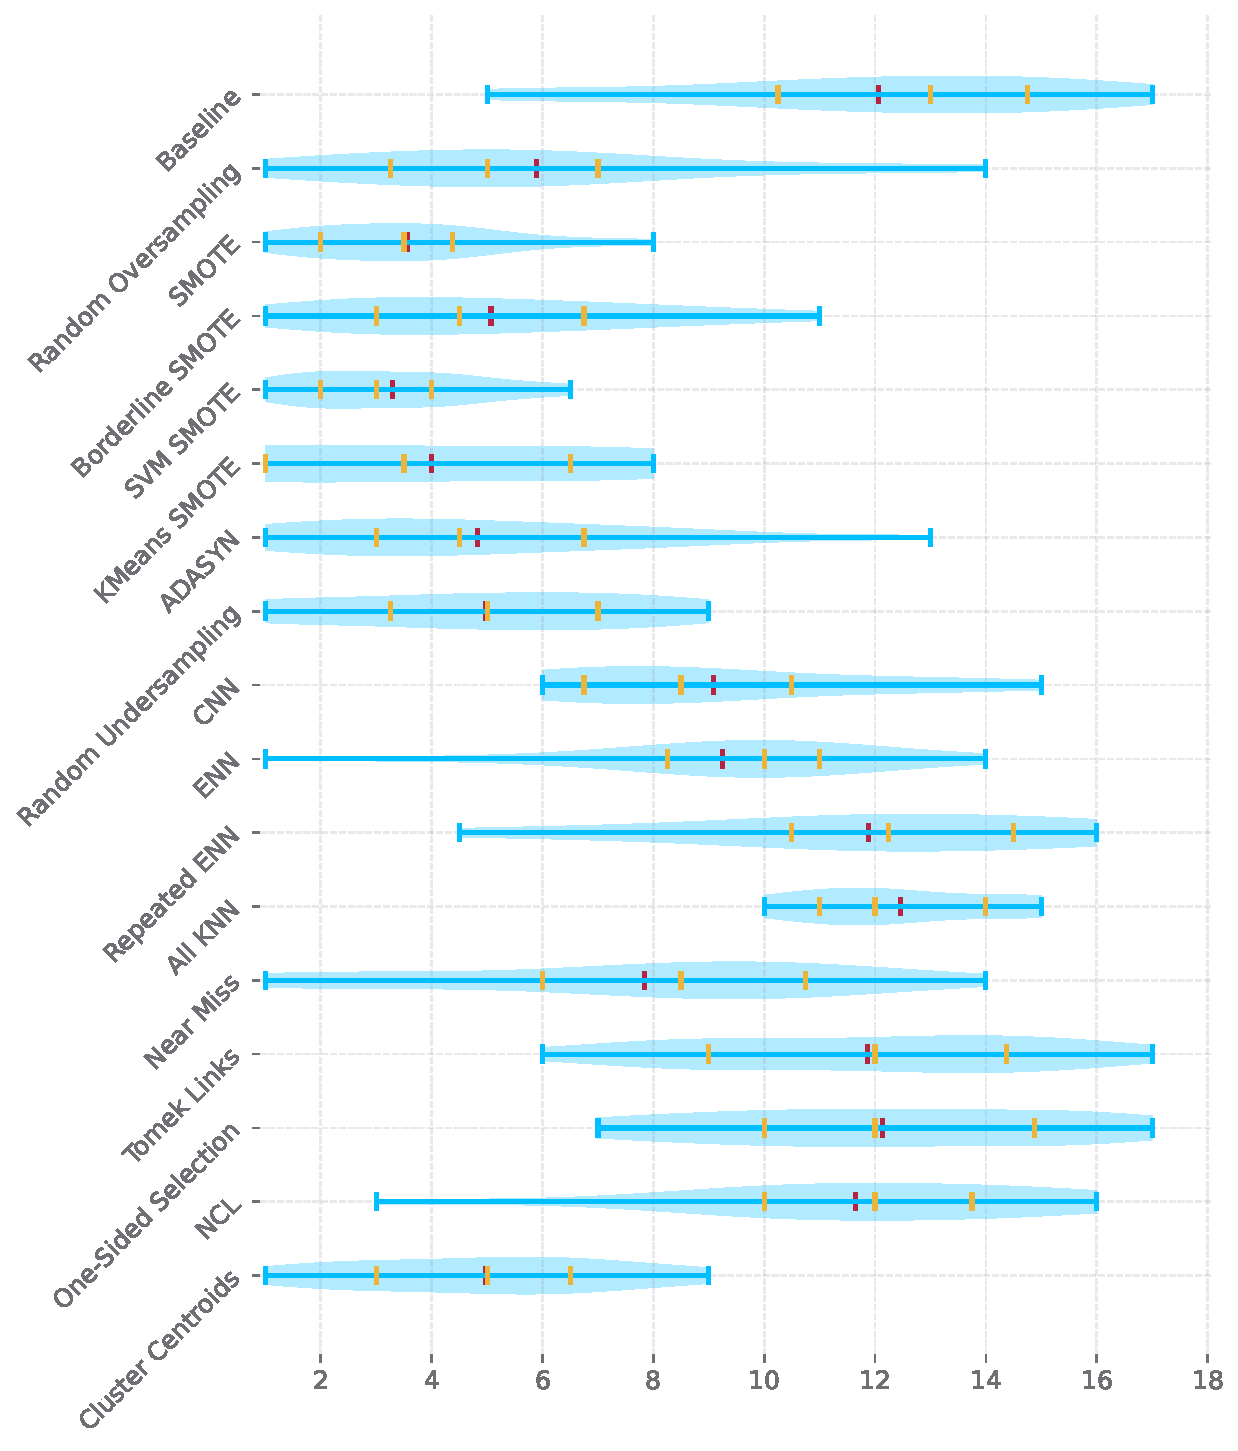
\includegraphics[width=\linewidth]{figures/partial_roc_auc_ranks_distribution.pdf}
    \caption{
        \textbf{Distribution of Ranks for Partial ROC AUC Evaluation Metric.} The figure shows the
        distribution of ranks computed across all datasets in the experiments. Ranks were computed
        from Partial ROC AUC scores for each preprocessing method separately. Red marks denote each
        method’s mean rank, and three yellow marks indicate the 25th, 50th and 75th percentiles.
    }
    \label{figure:p-roc-ranks}
\end{figure}

\begin{figure}
    \centering
    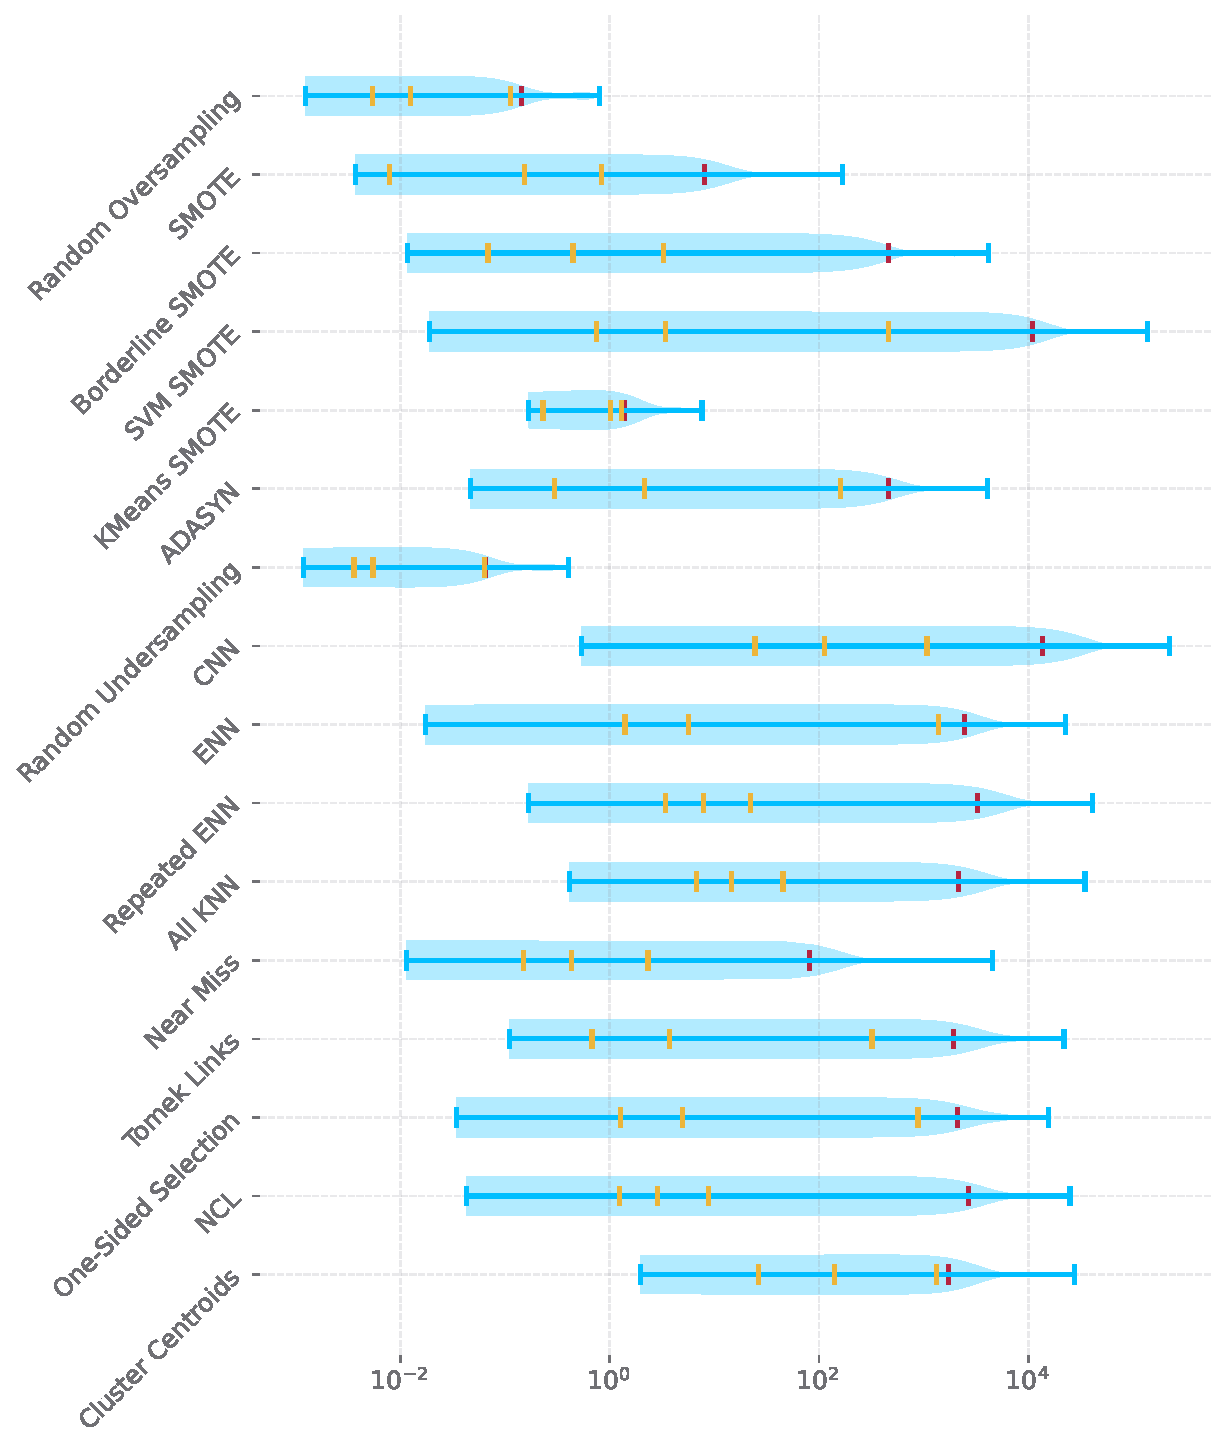
\includegraphics[width=\linewidth]{figures/preprocessing_times.pdf}
    \caption{
        \textbf{Distribution of Preprocessing Times Across All Datasets.} The figure shows the
        distribution of preprocessing times, in seconds, computed across all datasets in the
        experiment. Red marks denote each method's mean preprocessing time, and three yellow marks
        indicate the 25th, 50th and 75th percentiles.
    }
    \label{figure:preprocessing-times}
\end{figure}
